\subsection{Lower Bounds}\label{lb}


\begin{wrapfigure}{R}{0.5\textwidth}
\centering
\begin{subfigure}{.5\textwidth}
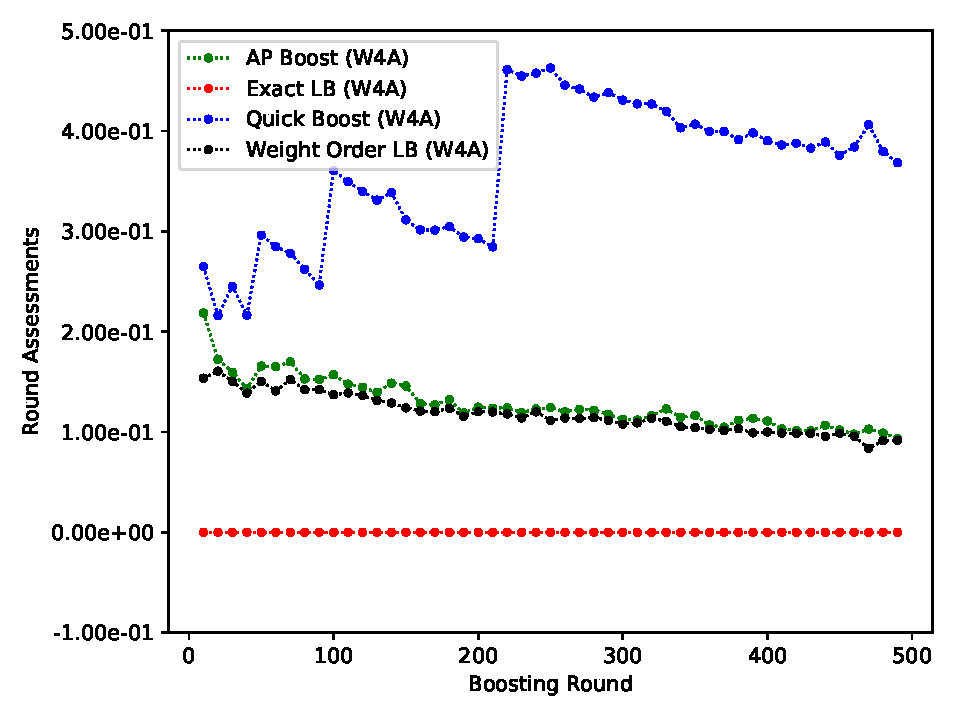
\includegraphics[width=\linewidth]{decisiontree/figures/result4_elb_w4a}
\end{subfigure}
\begin{subfigure}{.5\textwidth}
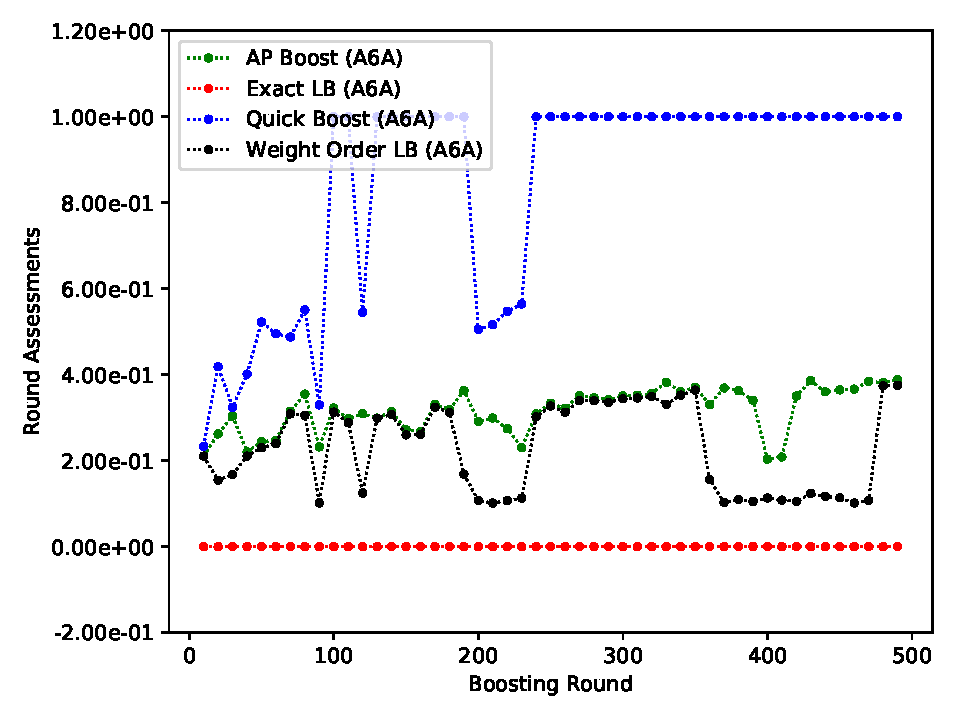
\includegraphics[width=\linewidth]{decisiontree/figures/result4_elb_a6a}
\end{subfigure}
\caption{Lower Bounds versus Upper Bounds. Datasets W4A (top) and A6A (bottom) were used with trees of depth 1.
The y-axis is the \emph{fraction of the gap}
between the exact lower bound
(at zero) and the full corpus size (at one) which an algorithm used in a
given round.
Non-cumulative example assessments are plotted for every 10 rounds.
}
\label{fig:elb}
\vspace{-2em}
\end{wrapfigure}



We compare \texttt{Adaptive-Pruning Boost} against two lower bounds, defined empirically based
on the boosting weights in a given round.
In our \emph{weight order lower bound}, we consider the minimum number
of examples required to determine that a given feature is underperforming
with the assumption that examples will be assessed in order of decreasing
boosting weight.
Our \emph{exact lower bound} permits examples to be assessed in any order,
and so bounds any possible algorithm which finds the best-performing feature.

\paragraph{Weight Order Lower Bound.}
For this bound, we first require that \texttt{Adaptive-Pruning Stump} selects the feature with
minimal error.
In the case of ties, an optimal feature may be chosen arbitrarily.
\texttt{Adaptive-Pruning Stump} need to assess every example for the returned
feature in order for \texttt{Adaptive-Pruning Boost} to calculate $\alpha$ and update weights $w$ , so the lower
bound for the returned feature is simply the total number of examples $n$.

Let $k^*$ be the returned feature, and $E^*$ its error rate
when assessed on all $n$ examples.
For any feature $k \ne k^*$ which is not returned, we need to prove that it is
underperforming (or tied with the best feature).
Let $J_k$ be the set of decision stumps which use feature $k$;
then we need to find the smallest value $m$ such that for all stumps
$j \in J_k$, we have $L^j_m \ge E^*$.
Our lower bound is simply 
$	LB_{wo} :=
	n + \sum_{k \ne k^*} \min \Set{m : \forall j \in J_k, L^j_{m} \ge E^*}$.
We present results in Figure~\ref{fig:wolb} showing that \texttt{Adaptive-Pruning Boost}
achieves this bound on a variety of datasets.
\texttt{Quick Boosting}, in contrast, sometimes approaches
this bound but often uses more examples than necessary.


\paragraph{Exact Lower Bound.}
In order to test the idea that adding examples in weight order is nearly optimal,
and to provide a lower bound on \emph{any} algorithm which finds the
optimal stump, we also present an exact lower bound on the problem.
Like the weight order lower bound, this bound is defined in terms of the boosting
weights in a given round; unlike it, examples may be assessed in any order.
It is not clear how one might achieve the exact lower bound without incurring an
additional cost in time.
We leave such a solution to future work.
However, we show in Figure~\ref{fig:elb} that this bound is, in fact,
very close to the weight order lower bound.

For the exact lower bound, we still require the selected feature $k^*$ to be
assessed against all examples; this is imposed by the boosting algorithm.
For any other feature $k \ne k^*$, we simply need the size of the smallest
set of examples which would prune the feature (or prove it is tied with $k^*$).
We will use $M \subseteq \Set{1,\dots,n}$ to denote a set of indexes of examples
assessed for a given feature,
and $L^j_M$ to denote the lower bound of stump $j$ when assessed on the
examples in subset $M$.
This bound, then, is
%\begin{align}
$	LB_{exact} :=
	n + \sum_{k \ne k^*} \min_{M : L^j_M \ge E^*} |M|$.
%\end{align}

We identify the examples included in the smallest subset $M$
for a given feature $k \ne k^*$ using integer linear programming.
We define binary variables $c_1,\dots,c_n$, where $c_i$ indicates whether example
$i$ is included in the set $M$.
We then create a constraint for each stump $j \in J_k$ defined for feature $k$
which requires that the stump be proven underperforming.
Our program, then, is:
$
%\begin{align}
	\texttt{Minimize } 
%	&
%	\\ \nonumber
%	 & 
	 \sum_{i=1}^n c_i
%	\\ \nonumber
	\texttt{ s.t. }
%	& 
	c_i \in \Set{0,1}
		~~~ \forall i 
%		\in \Set{1,\dots,n}
, \texttt{ and }
%	\\ \nonumber
%	& 
	\sum_{i=1}^n c_i w_i \1{ h_j(x_i) \ne y_i }
		\ge E^*
		~~~ \forall j \in J_k$.
%\end{align}

\paragraph{Discussion.}
Figure~\ref{fig:elb} shows a non-cumulative comparison of our weight order lower bound to the global lower bound. Minimizing the global lower bound function mentioned above is computationally expensive. For this reason we used binary class datasets of moderate size and trees of depth 1 as weak leaners, but we have no reason to believe that the technique would not work for deeper trees and multi-class datasets. Refer to Table~\ref{datasets} for details of datasets.
The weight order lower bound and \texttt{Adaptive-Pruning Boost} 
are within 10-20\% of the exact lower bound,
but \texttt{Quick Boost} often uses half to all of the unnecessary
training examples in a given round.